\chapter{Teória}
\label{part:teoria}

V teoretickej časti si rozoberieme najpoužívanejšie riadenie s optimalizáciou, čo je prediktívne riadenie založené na modeli. Vysvetlíme si spôsob jeho použitia a rozdiel medzi lineárnym a nelineárnym riadením. Druhá polovica teoretickej časti bude venovaná distribuovanému optimalizačnému algoritmu, ktorý bude v práci využívaný a ukážeme, ako môžeme využiť tento algoritmus pri riešení prediktívneho riadenia.

\section{Prediktívne riadenie}
\label{se:teoriaMPC}

Prediktívne riadenie, pod anglickou skratkou MPC, je známe už od minulého storočia. Je jednou z najpoužívanejších foriem riadenia s optimalizáciou. Dokáže zvládať mnohorozmerné riadenie, jedna z jeho najväčších výhod je, že doň vieme zahrnúť ohraničenie. Tým poskytuje obrovskú prevahu oproti svojmu predchodcovi, lineárnemu kvadratickému regulátoru, inak LQR. 

Základnou myšlienkou MPC je, že pomocou známeho matematického modelu systému vieme predikovať budúce správanie sa procesu na pevne určenom časovom horizonte. Tieto informácie vieme využiť pri výpočte optimálnych akčných zásahov, pomocou minimalizácie účelovej funkcie. Takto navrhnuté riadenie nám zabezpečuje garanciu dodržania všetkých ohraničení.

\subsection{Formulácia MPC}
\label{subse:MPC}
Ako sme už spomínali v rámci MPC je nutné poznať matematický model reprezentujúci riadený systém, či už v lineárnej alebo nelineárnej podobe. Najčastejšie sa používa lineárny model v tvare diskrétnej stavovej rovnice v nasledovnej podobe
\begin{align}
	x_{k+1} = Ax_{k} + Bu_{k}\\
	y_{k} = Cx_{k} + Du_{k}
\end{align}
kde $x$ predstavuje stĺpcový vektor stavov o veľkosti $n_{x}$, $u$ predstavuje stĺpcový vektor vstupov o veľkosti $n_{u}$, $A$ je matica stavov definovaná ako $A \in {\rm I\!R}^{n_{x}\times n_{x}}$, B je matica vstupov definovaná ako $B \in {\rm I\!R}^{n_{u}\times n_{u}}$. Rovnicu (2.2), ktorá predstavuje rovnicu výstupu zo systému môžme pri návrhu MPC zanedbať, budeme totiž brať do úvahy iba stavové riadenie.

Základnú formuláciu lineárneho MPC si zadefinujeme nasledovne
\label{math:LinearneMPC}
\begin{subequations}
	\begin{align}
		\displaystyle \min_{u_0,...,u_{N-1}} \hspace{0.1cm} & 
		\sum_{k=1}^{N}\norm{Qx_k}^{2}_{2}+\sum_{k=0}^{N-1}\norm{Ru_k}^{2}_{2}\\
		\textrm{s.t.} \hspace{0.5cm} & x_{k+1} = Ax_{k}+Bu_{k}\hspace{0.5cm} k=0,\dots,N-1\\
		& x_{0} = x(t)\\
		& \underline{x} \leq x_{k} \leq \overline{x}\hspace{0.5cm} k=0,\dots,N\\
		& \underline{u} \leq u_{k} \leq \overline{u}\hspace{0.5cm} k=0,\dots,N-1
	\end{align}
\end{subequations}
kde matica $Q$ predstavuje váhovú maticu stavov definovanú ako $Q \in {\rm I\!R}^{n_{x}\times n_{x}}$, matica $R$ je váhová maticu vstupov definovaná ako $R \in {\rm I\!R}^{n_{u}\times n_{u}}$. Pomocou týchto váhových matíc si môžme nastavovať prioritu počas optimalizácie pre každý stav a vstup samostatne. 

\subsection{Lineárne riadenie s kompenzáciou nelinearity}
\label{subse:LinearneMPCKomp}
Najjednoduchšou formou prediktívneho riadenia je lineárne riadenie. V rámci MPC sa používa lineárny model s lineárnymi ohraničeniami. Ide o najmenej komplikovanú formu, ktorá má výhodu v krátkom výpočtovom čase, čo sa môže hodiť pri systémoch s rýchlou dynamikou. Keďže všetko je vždy o kompromisoch a za rýchlym výpočtovým časom je veľa zanedbaní, ktoré sú najmä v lineárnom modeli. V realite sa málokedy stretneme so systémom, ktorý by stačilo opísať jednoduchým stavovým modelom a riadenie by fungovalo bezchybne. 
\begin{figure}[H]
	\centering
	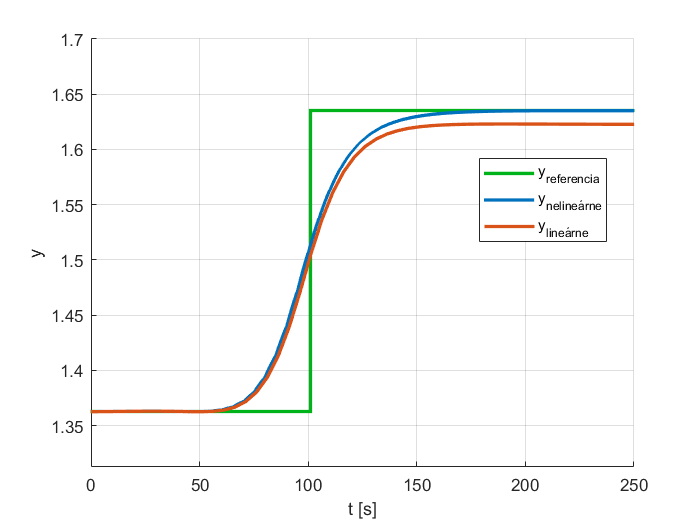
\includegraphics[width=11cm,height=8cm]{images/linear_vs_nonlinear}
	\caption{Rozdiel medzi lineárnim a nelineárnim riadením}
\end{figure}
Pri takomto riadení vznikajú trvalé regulačné odchýlky (Obr.2.1). Aby sa tomu predišlo, musia sa pridávať doplnkové opatrenia, ktoré by vyrovnávali nelinearitu. 

Jedným z najefektívnejších je pridať integračné vlastnosti regulátoru. Pomocou nich bude regulátor minimalizovať rozdiel medzi nelineárnym procesom a lineárnym modelom procesu. Jednoducho sa pridá do lineárneho modelu porucha, ktorá bude reprezentovať tento rozdiel. Takže rovnicu (2.1) nahradíme novým systémom, rozšíreným o poruchu.
\begin{align}
	x_{k+1} &= Ax_{k} + Bu_{k} + Ed_{k}\\
	d_{k+1} &= d_{k}
\end{align}
Nastáva problém, odkiaľ sa získajú aktuálne hodnoty poruchy, reprezentujúcej odchýlku od nelinearity. Takýto člen sa nedá priamo merať senzorom, dá sa ale získať pomocou odhadu. Môžeme využiť buď Luenbergerov pozorovateľ, alebo pokročilejší, časovo premenný Kalmanov filter. 

Výsledná forma takto zadefinovaného MPC bude v nasledovnom tvare.
\begin{subequations}
	\begin{align}
	\displaystyle \min_{u_0,...,u_{N-1}} \hspace{0.1cm} & 
	\sum_{k=1}^{N}\norm{Qx_k}^{2}_{2}+\sum_{k=0}^{N-1}\norm{Ru_k}^{2}_{2}\\
	\textrm{s.t.} \hspace{0.5cm} & x_{k+1} = Ax_{k} + Bu_{k} + E\hat{d}_{k}\hspace{0.5cm} k=0,\dots,N-1\\
	& x_{0} = x(t)\\
	& \hat{d}_{0} = \hat{d}(t)\\
	& \underline{x} \leq x_{k} \leq \overline{x}\hspace{0.5cm} k=0,\dots,N\\
	& \underline{u} \leq u_{k} \leq \overline{u}\hspace{0.5cm} k=0,\dots,N-1
	\end{align}
\end{subequations}
kde $\hat{d}$ predstavuje rozdiel medzi lineárnym a nelineárnym modelom systému, $E$ je jednotková matica definovaná ako $E \in {\rm I\!R}^{n_{x}\times n_{x}}$.

\subsection{Nelineárne riadenie}
\label{subse:NelinearneMPC}
Ak by sme chceli predísť všetkým prídavkom k lineárnemu riadeniu a následnému ladeniu všetkých pridaných váhových matíc, je možnosť priamo vymeniť lineárny model za nelineárny. V rámci tejto práce sa budeme venovať práve takémuto nelineárnemu riadeniu, tak, že nahradíme lineárny model používaný v MPC priamo za nelineárny.

Nelineárne rovnice budú vo forme diferenciálnych rovníc, ktoré následne diskretizujeme v rámci periódy vzorkovania systému. Takto získanú rovnicu použijeme miesto stavového opisu a výsledné MPC bude mať nasledovnú formu.
\begin{subequations}
	\begin{align}
	\displaystyle \min_{u_0,...,u_{N-1}} \hspace{0.1cm} & 
	\sum_{k=1}^{N}\norm{Qx_k}^{2}_{2}+\sum_{k=0}^{N-1}\norm{Ru_k}^{2}_{2}\\
	\textrm{s.t.} \hspace{0.5cm} & x_{k+1} = f(x_{k},u_{k},T_{s})\hspace{0.5cm} k=0,\dots,N-1\\
	& x_{0} = x(t)\\
	& \underline{x} \leq x_{k} \leq \overline{x}\hspace{0.5cm} k=0,\dots,N\\
	& \underline{u} \leq u_{k} \leq \overline{u}\hspace{0.5cm} k=0,\dots,N-1
	\end{align}
\end{subequations}
Takýto prístup môže spôsobiť komplikácie pri riešení MPC. Výrazne sa zväčší výpočtový čas a je komplikovanejšie s ním narábať. Cieľom tejto práce bude zrýchliť aj takéto riadenie tak, aby ho bolo možné využiť pri systémoch s rýchlou dynamikou.


\section{Eulerova metóda diskretizácie}
\label{se:diskretizacia}
Táto metóda je stará už vyše 200 rokov, ale aj napriek tomu sa používa dodnes. Je založená na numerickej diskretizácii. Chyba, ktorej sa dopúšťame použitím tejto metódy, je priamo úmerná kroku diskretizácie, ktorý zvolíme. Nie je až taká účinná v porovnaní s ostatnými metódami, ale je používaná ako základ komplexnejších metód. Pre účely nášho projektu bude postačujúca v základnej forme a jej jednoduchosť bude pre nás výhodou.

Majme nasledovnú vzťah:
\begin{align}
		\dot{x}(t) &= f(x,t),
\end{align}
kde $\dot{x}(t)$ predstavuje diferenciálnu rovnicu $\dot{x}(t)=\frac{dx(t)}{dt}$, ktorá opisuje modle systému v kontinuálnom čase. Pomocou Eulerovej metódy ju môžeme nasledovne pretransformovať:
\begin{align}
	x_{k+1} &= x_{k} + hf(x_{k}),
\end{align}
kde h predstavuje dĺžku kroku, v našom projekte bude rovnaká, ako perióda vzorkovania diskretizovaného systému.
\begin{figure}[H]
	\centering
	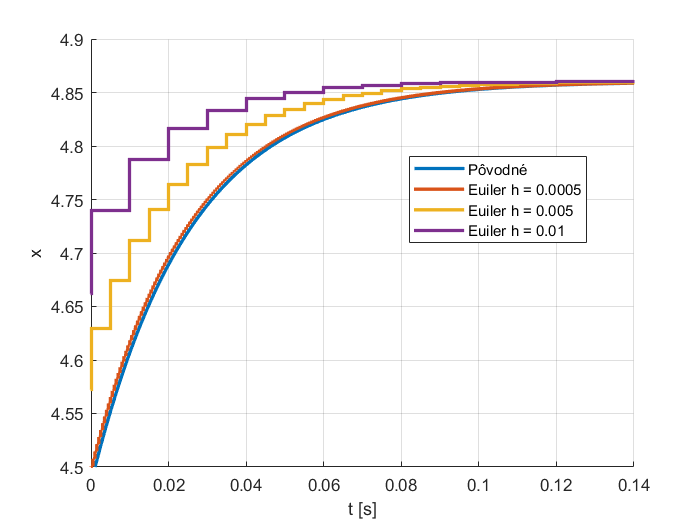
\includegraphics[width=11cm,height=8cm]{images/Euler_method}
	\caption{Eulerová diskretizácia}
\end{figure}
Ako môžeme vidieť na (Obr. 2.1), čím budeme používať menšiu periódu, tým presnejšia bude diskretizácia.


\section{Decentralizovaná optimalizácia}
\label{se:DecentralizovanaOptimalizacia}
Zvyčajne, pri všeobecnej optimalizačnej úlohe, si ako prvé zadefinujeme účelovú funkciu, určíme si začiatočné podmienky a ohraničenia potom zvolíme vhodnú optimalizačnú metódu pre nájdenie optima. Takto formulovanú optimalizáciu nazývame centralizovaná optimalizácia, kde sa všetky premenné nachádzajú pod jedným problémom a výsledkom je centralizované riešenie. 
\begin{subequations}
	\begin{align}
		\displaystyle \min_{x} \hspace{0.5cm} & 
		f(x)\\
		\textrm{s.t.} \hspace{0.5cm} & Lx = v
	\end{align}
\end{subequations}
V tejto práci ale využijeme takzvanú decentralizáciu optimalizačného problému. Optimalizačnú úlohu si rozložíme na viacero častí $ f(x) = g(z) + h(y)$ a každú riešime samostatne. Výsledkom bude viacero decentralizovaných riešení.
\begin{subequations}
	\begin{align}
		\displaystyle \min_{} \hspace{0.5cm} & 
		g(z) + h(y)\\
		\textrm{s.t.} \hspace{0.5cm} & L_{1}z = v_1\\
		& L_{2}y = v_2
	\end{align}
\end{subequations}
Takéto rozloženie účelovej funkcie na viac častí umožňuje zjednodušenie optimalizačnej úlohy a pri riešení náročných optimalizácií môže výrazne skrátiť čas výpočtu.
\begin{figure}[H]
	\centering
	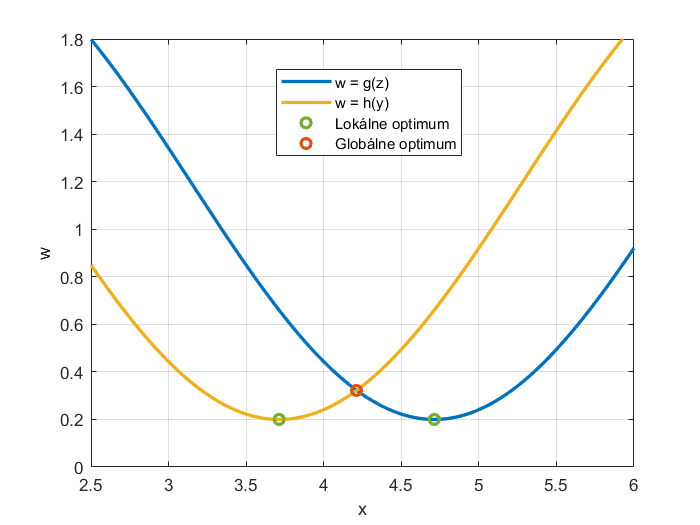
\includegraphics[width=11cm,height=8cm]{images/Global_Local_ADM}
	\caption{Porovnanie globálneho a lokálneho riešenia}
\end{figure}
Jedným z problémov, ktorý môže nastať pri decentralizovanej optimalizácií je, že jednotlivé decentrálne riešenia môžu uviaznuť vo svojich lokálnych optimách (Obr. 2.3). Cieľom decentralizovanej optimalizácie bude aj, aby jednotlivé riešenia nekonvergovali do lokálneho, ale do jedného globálneho. 
\subsection{ADMM}
\label{subse:ADMM}
ADMM je skratka z anglického názvu (Alternating Direction Method of Multipliers). Pomocou tejto metódy vieme riešiť decentralizovaný optimalizačný problém.
Formulácia optimalizačného problému pre ADMM je v nasledovnom tvare
\begin{subequations}
	\begin{align}
		\displaystyle \min_{y,z} \hspace{0.5cm} & 
		g(z) + h(y),\\
		\textrm{s.t.} \hspace{0.5cm} & H_{1}z + H_{2}y = b,
	\end{align}
\end{subequations}
kde $y$ a $z$ sú optimalizované premenné, ktoré sú definované nasledovne $y \in {\rm I\!R}^n $, $ z\in {\rm I\!R}^m$. Rovnica (2.12b) predstavuje novú podmienku, ktorá prepája decentralizované premenné, matica $H_{1}$, $H_{2}$ a vektor $b$ sú skonštruované tak, aby podmienky boli vhodné pre všetky prípady, ich rozmery sú $H_{1} \in {\rm I\!R}^{p \times n}$, $H_{2} \in {\rm I\!R}^{p \times m}$ a teda vo výsledku je vektor $b \in {\rm I\!R}^p $. 

Ako môžeme vidieť, rozdiel medzi decentralizovaným a centralizovaným optimalizačným problémom je, že sme rozdelili optimalizované premenné, spolu s účelovou funkciou, ktorá musí umožňovať takéto rozdelenie premenných. S takýmto rozdelením nám zároveň pribudla nová podmienka do optimalizačného problému, ktorá prepája rozdelenú funkciu. Táto podmienka sa nazýva duálna funkcia. 
Ďalej môžeme pokračovať tak, že túto novú podmienku pridáme do optimalizačného problému pomocou Lagrangeovej metódy a vytvoríme rozšírený lagrangeán.
\begin{equation}
	\mathcal{L}_{\rho} = g(z) + h(y) + \lambda^{T}\left(  H_{1}z + H_{2}y - b \right) + \frac{\rho}{2} \norm{H_{1}z + H_{2}y - b}_{2}^{2}
\end{equation}
Rozšírenie lagrangeánu predstavuje posledný člen $\frac{\rho}{2} \norm{H_{1}z + H_{2}y - b}_{2}^{2}$ a zabezpečuje, aby bola funkcia spojite diferencovateľná a zároveň pomáha konvergencii. Pridaním tohoto člen neovplyvníme hodnotu optima, keďže je v optime nulové. Takto definovanú úlohu vieme riešiť separátnym prístupom k jednotlivým premenným lagrangianu $\mathcal{L}_{\rho} \left(z,y,\lambda \right)$
\label{math:ADMM_iteracie}
\begin{align}
	&z^{(i+1)} = \argmin_{z} \mathcal{L}_{\rho} \left(z,y^{i},\lambda^{i} \right),\\
	&y^{(i+1)} = \argmin_{y} \mathcal{L}_{\rho} \left(z^{i},y,\lambda^{i} \right),\\
	&\lambda^{(i+1)} = \lambda^{i} + \rho( H_{1}z^{(i+1)} + H_{2}y^{(i+1)} - b ),
\end{align}
kde $\rho > 1$. Táto iteračná metóda prebieha v takzvanom duálnom framworku, ktorý sa skladá z primárneho problému (minimalizácia $z$, minimalizácie $y$) a aktualizácie duálneho problému $\lambda$. V poslednom vzťahu, kde sa aktualizuje duálna premenná, je aplikovaný podobný postup ako v numerickej gradientovej metóde, ale vykoná sa iba raz, $\rho$ tu predstavuje dĺžku kroku. Funkcia tohoto duálneho problému je konkávna, a teda sa ľahko maximalizuje, čo nespôsobuje ťažkosti, ak náš primárny problém je konvexný. Ak primárny problém spĺňa konvexnosť tak jeho minimum korešponduje s maximom duálneho problému. Preto neoptimalizujeme v smere poklesu (ako tomu je pri minimalizácii v gradientovej metóde), ale hýbeme sa v smere rastu\cite{bib1}. 
\label{subse:ADMM2}

Postup pri iterácií v ADMM.
\begin{description}
	\item[Krok 1:] {Paralelne vyriešime minimalizáciu lagrangeana vzhľadom k všetkým predikčným horizontom, \hyperref[math:ADMM_iteracie]{rovnice (2.14,2.15)}.}
	\item[Krok 2:] {Aktualizujeme duálny parameter $\lambda$ s novými hodnotami, \hyperref[math:ADMM_iteracie]{rovnica (2.16)}.}
	\item[Krok 3:] {Opakujeme od kroku 1, až kým skonvergujeme do globálneho minima (narazíme na zastavovacie kritérium).}
\end{description}



\section{Prediktívne riadenie pomocou ADMM}
\label{se:MPC_ADMM}
V tejto časti teórie spojíme \hyperref[subse:MPC]{MPC(2.1.1)} a \hyperref[subse:ADMM]{ADMM (2.4)}. Najskôr aplikujeme ADMM na lineárnom riadení, ukážeme si ako rozložiť MPC podla predikčných horizontov a vysvetlíme si spôsob, akým budeme získavať optimálne decentralizované riešenia. V druhej časti si ukážeme, čo všetko musíme nahradiť a upraviť, aby sme boli schopní použiť ADMM pri nelineárnom riadení. 

\subsection{Linearne prediktívne riadenie}
\label{subse:Lin_MPC_ADMM}
Ako sme už spomínali, v tejto časti využijeme ADMM pre lineárne riadenie. Takže naším cieľom bude overiť funkčnosť paralelného riešenia decentralizovaného optimalizačného problému so snahou zrýchliť výpočet MPC. Myšlienka spočíva v rozdelení MPC na $N$ predikčných horizontov a následné paralelné riešenie decentralizovaného MPC. Tento výpočet bude prebiehať na viacerých počítačoch, ktoré budú hľadať centralizované riešenie. 

Majme linearne MPC bez ohraničení:
\label{math:2.14}
\begin{subequations}
	\begin{align}
		\displaystyle \min_{u_0,...,u_{N-1}} \hspace{0.1cm} & 
		\sum_{k=1}^{N}\norm{Qx_k}^{2}_{2}+\sum_{k=0}^{N-1}\norm{Ru_k}^{2}_{2},\\
		\textrm{s.t.} \hspace{0.5cm} & x_{k+1} = Ax_{k}+Bu_{k}\hspace{0.5cm} k=0,\dots,N-1,\\
		& x_{0} = x(t).
	\end{align}
\end{subequations}
Postupujeme podla teórie uvedenej v \hyperref[subse:ADMM]{(2.4)}. Takto formulované MPC si môžeme rozdeliť na $2,\dots,N$ decentralizovaných problémov. Budeme pracovať s úplnou decentralizáciou a MPC si rozdelíme na $N$ decentralizovaných optimalizačných problémov.
\label{math:ADMM_MPC}
Ako príklad si zoberme MPC pre predikčný horizont $N = 3$:
\begin{subequations}
	\begin{align}
		\displaystyle\min_{u_0,u_1,u_2}\hspace{0.1cm}&\norm{Qx_1}^{2}_{2}+\norm{Qx_2}^{2}_{2}+\norm{Qx_3}^{2}_{2}+\norm{Ru_0}^{2}_{2}+\norm{Ru_1}^{2}_{2}+\norm{Ru_2}^{2}_{2},\\
		& x_{0} = x(t),\\
		&x_{1} = Ax_{0}+Bu_{0},\\
		&x_{2} = Ax_{1}+Bu_{1},\\
		&x_{3} = Ax_{2}+Bu_{2}.
	\end{align}
\end{subequations}
Za každý stav si môžeme dosadiť model systému v príslušnom kroku $k=1,\dots,3$:
\begin{subequations}
	\begin{align}	
	\begin{split}			
			\displaystyle\min_{u_0,u_1,u_2}\hspace{0.1cm}&\norm{Q(Ax_{0}+Bu_{0})}^{2}_{2}+\norm{Ru_0}^{2}_{2}+\norm{Q(Ax_{1}+Bu_{1})}^{2}_{2}+\norm{Ru_1}^{2}_{2}+\\
			&\norm{Q(Ax_{2}+Bu_{2})}^{2}_{2}+\norm{Ru_2}^{2}_{2}
	\end{split}\\
	& x_{0} = x(t).
	\end{align}
\end{subequations}
Teraz máme optimalizačný problém, ktorý chceme optimalizovať pre každý predikčný horizont samostatne. Takže pre každý stav musíme poznať počiatočné podmienky ($x_0,x_1,x_2$). V našom prípade máme počiatočné podmienky iba pre prvý stav, rovnica (2.16b), čiže ostatné musíme hľadať. Práve k tomu nám dopomôže duálna funkcia, ktorá bude koordinovať hľadané počiatočné stavy s ich skutočnými hodnotami. 

Duálna funkcia bude vychádzať z modelu systému \hyperref[math:2.14]{(2.14b)} a prepíšeme si ju do nasledovnej podoby:
\begin{align}
	H_{1}u_{k-1} + H_{2}x_{k} = -Ax_{k-1},
\end{align}
kde $H_{1} = B$ a je definované ako $H_{1} \in {\rm I\!R}^{n_{u}\times n_{u}}$, $H_{2}$ je záporná jednotková matica definovaná ako $H_{2} \in {\rm I\!R}^{n_{x}\times n_{x}}$. Pridáme túto duálnu funkciu do nášho všeobecného optimalizačného problému:
\begin{subequations}
	\begin{align}
		\displaystyle \min_{u_0,...,u_{N-1},x_1,...,x_N} \hspace{0.1cm} & 
		\sum_{k=1}^{N}
		\norm{Qx_k}^{2}_{2}+\sum_{k=0}^{N-1}\norm{Ru_k}^{2}_{2},\\
		\textrm{s.t.} \hspace{1.1cm} & x_{n+1} = Ax_{k}+Bu_{k} \hspace{0.5cm} k=0,\dots,N-1,\\
		& x_{0} = x(t),\\
		&H_{1}u_{k-1} + H_{2}x_{k} = -Ax_{k-1}\hspace{0.5cm} k=1,\dots,N.
	\end{align}
\end{subequations}
Pomocou upravenej Lagrangianovej metódy sa zbavíme duálnej funkcie (2.21d) a vytvoríme rozšírenú Lagrangianovú funkciu:
\label{math:RozsirenyLag}
\begin{equation}
\begin{split}
\mathcal{L}_{\rho} =&~ \sum_{k=0}^{N-1}\norm{Q(Ax_{k}+Bu_{k})}^{2}_{2}+\sum_{k=0}^{N-1}\norm{Ru_k}^{2}_{2} +\\+&~\sum_{k=1}^{N-1}\lambda_{k}^{T}\left(  H_{1}u_{k-1} + H_{2}x_{k} + Ax_{k-1}\right) +\\+&~\sum_{k=1}^{N-1}\frac{\rho}{2} \norm{H_{1}u_{k-1} + H_{2}x_{k} + Ax_{k-1}}_{2}^{2}
\end{split}
\end{equation}
Pre zjednodušenie využijeme substitúciu pre jednotlivé premenné našej optimalizácie:
\begin{align}
	U_{0} =\begin{bmatrix}
	u_{0}\\
	x_{0}
	\end{bmatrix},
	U_{1} =\begin{bmatrix}
	u_{1}\\
	x_{1}
	\end{bmatrix}, \dots ,
	U_{k} =\begin{bmatrix}
	u_{k}\\
	x_{k}
	\end{bmatrix}.
\end{align}
Dosadíme jednotlivé substituované premenné do rovnice \hyperref[math:RozsirenyLag]{(2.19)}, rozšírime si matice vzhľadom k substituovaným premenným a dostaneme nasledovný vzťah:
\label{math:RozsirenyLag2}
\begin{equation}
\begin{split}
\mathcal{L}_{\rho} =&~ \sum_{k=0}^{N-1}\norm{\tilde{Q}(\tilde{A}U_{k}+\tilde{B}U_{k})}^{2}_{2}+\sum_{k=0}^{N-1}\norm{\tilde{R}U_k}^{2}_{2} +\\&~\sum_{k=1}^{N-1}\lambda_{k}^{T}\left(  \tilde{H}_{1}U_{k-1} + \tilde{H}_{2}U_{k} + \tilde{A}U_{k-1} \right) +\\&~\sum_{k=1}^{N-1}\frac{\rho}{2} \norm{\tilde{H}_{1}U_{k-1} + \tilde{H}_{2}U_{k} + \tilde{A}U_{k-1}}_{2}^{2}
\end{split}
\end{equation}
kde $U$ je definované ako $U \in {\rm I\!R}^{p\times1}, p = n_{x} + n_{u}$, počet rovníc je $r$, potom všetky rozšírené matice sú definované ako $(\tilde{A}$, $\tilde{B}$, $\tilde{Q}$, $\tilde{R}$, $\tilde{H}_{1}$, $\tilde{H}_{2}) \in {\rm I\!R}^{r \times p}$.
 Jednotlivé rozšírené matice sú zložené nasledovne:
\begin{subequations}
	\begin{align}
		&\tilde{A} = \begin{bmatrix}
						0\\
						A
					\end{bmatrix},\\
		&\tilde{B} = \begin{bmatrix}
							B & 0
					 \end{bmatrix},\\
		&\tilde{Q} = \begin{bmatrix}
						0 & Q
					 \end{bmatrix},\\
		&\tilde{R} = \begin{bmatrix}
						R & 0
					\end{bmatrix},\\
		&\tilde{H}_{1} = \begin{bmatrix}
							B & 0
						\end{bmatrix},\\
		&\tilde{H}_{2} = \begin{bmatrix}
							0 & -I
						\end{bmatrix}.
	\end{align}
\end{subequations}
\label{math:Linear_Lagrangean}\noindent
Ako môžeme vidieť, takto upravenú Lagrangianovú funkciu môžeme jednoducho optimalizovať vzhľadom k jednotlivým krokom predikčného horizontu:
\begin{subequations}
	\begin{align}
	&u_{0}^{(i+1)} = \argmin_{u_{0}} \mathcal{L}_{\rho} \left(u_{0},x_{0},x_{1}^{i},\lambda_{1}^{i}\right)\\
	&U_{k}^{(i+1)} = \argmin_{U_{k}} \mathcal{L}_{\rho} \left(U_{k},U_{k-1}^{i},\lambda_{k}^{i},U_{k+1}^{i},\lambda_{k+1}^{i}\right) \hspace{0.5cm} k=1,\dots,N-2\\
	&U_{k}^{(i+1)} = \argmin_{U_{k}} \mathcal{L}_{\rho}\left(U_{k},U_{k-1}^{i},\lambda_{k}^{i}\right) \hspace{0.5cm} k=N-1\\
	&\lambda_{k}^{(i+1)} = \lambda_{k}^{i} + \rho( \tilde{H}_{1}U_{k-1}^{(i+1)} + \tilde{H}_{2}U_{k}^{(i+1)} - \tilde{A}U_{k-1})\hspace{0.5cm} k=1,\dots,N-1
	\end{align}
\end{subequations}
Postup pri iterácií v ADMM sme si vysvetlili v kapitole \hyperref[subse:ADMM2]{(2.4)}. Keďže pracujeme s lineárnym modelom, pre minimalizáciu Lagrangianovej funkcie sme si zvolili analytickú metódu optimalizácie. Nájdeme teda gradient Lagrangianovej funkcie vzhľadom k optimalizovanej premennej, položíme ho rovný nule a vyjmeme si optimalizovanú premennú:
\begin{align}
&\frac{\partial \mathcal{L}_{\rho}}{\partial U_{k}} = 0  \hspace{0.5cm} \Longrightarrow  \hspace{0.5cm} U_{k}^{*}.
\end{align}
Vzhľadom na to, že používame analytické riešenie optimalizácie, môžeme nájsť všeobecné vzťahy, ktoré budú vždy platné.
Máme tri prípady, ktoré môžu nastať \hyperref[math:Linear_Lagrangean]{rovnice (2.31a,2.31b,2.31c)}
\begin{enumerate}
	\item{Prvý krok predikčného horizontu $k = 0$, v tomto prípade musíme urobiť výnimku, keďže derivácia podla konštanty $x_0$ je nulová, teda nemôžme použiť rozšírenú formu Lagrangianovej funkcie \hyperref[math:RozsirenyLag]{(2.21)}, ale využijeme jej základnú formu  \hyperref[math:RozsirenyLag]{(2.19)}:\\
		\begin{subequations}
			\begin{align}
				\begin{split}
					&\mathcal{L}_{\rho} =\norm{Q(Ax_{0}+Bu_{0})}^{2}_{2}+\norm{Ru_{0}}^{2}_{2} +\lambda_{1}^{T}\left(H_{1}u_{0} + H_{2}x_{1} + Ax_{0} \right)+\\&\hspace{0.8cm}\norm{H_{1}u_{0} + H_{2}x_{1} + Ax_{0}}_{2}^{2}+\dots
				\end{split}\\
				&\frac{\partial \mathcal{L}_{\rho}\left(u_{0},x_{0},x_{1}^{i},\lambda_{1}^{i}\right)}{\partial u_{0}} = 0,\\
				&u_{0}^{*} = -M_{0}^{-1}\left(2B^{T}Q^{T}QAx_{0}+H_{1}^{T}(\lambda_{1}^{i}+\rho H_{2}x_{1}^{i}+\rho Ax_{0})\right),\\
				&M_{0} = 2B^{T}Q^{T}QB + 2R^{T}R +\rho H_{1}^{T}H_{1}.
			\end{align}
		\end{subequations}
	}
	\item{Keď krok predikčného horizontu $k$ sa nachádza v otvorenom intervale $\left(0,N-1\right)$:\\
		\begin{subequations}
			\begin{align}
				&\frac{\partial \mathcal{L}_{\rho}\left(U_{k},U_{k-1}^{i},\lambda_{k}^{i},U_{k+1}^{i},\lambda_{k+1}^{i}\right)}{\partial U_{k}} = 0,\\
				&U_{k}^{*} = -M_{n}^{-1}\left(\tilde{H}_{2}^{T}f_{1}(\lambda_{k}^{i},U_{k-1}^{i})+(\tilde{H}_{1}^{T}+\tilde{A}^{T})f_{2}(\lambda_{k+1}^{i},U_{k+1}^{i})\right),\\
				\begin{split}
					& M_{n} = 2\tilde{A}^{T}\tilde{Q}^{T}\tilde{Q}\tilde{A}+2\tilde{A}^{T}\tilde{Q}^{T}\tilde{Q}\tilde{B}+2\tilde{B}^{T}\tilde{Q}^{T}\tilde{Q}\tilde{B}+2\tilde{B}^{T}\tilde{Q}^{T}\tilde{Q}\tilde{A}+\\
					&\hspace{1.0cm}2\tilde{R}^{T}\tilde{R} + \rho\tilde{H}_{2}^{T}\tilde{H}_{2}+ \rho\tilde{H}_{1}^{T}\tilde{H}_{1} + \rho\tilde{H}_{1}^{T}\tilde{A} + \rho\tilde{A}^{T}\tilde{H}_{1}+ \rho\tilde{A}^{T}\tilde{A}
				\end{split}\\
				& f_{1}(\lambda_{k}^{i},U_{k-1}^{i}) = \lambda_{k}^{i} + \rho\tilde{H}_{1}U_{k-1}^{i}+\rho\tilde{A}U_{k-1}^{i},\\
				& f_{2}(\lambda_{k+1}^{i},U_{k+1}^{i}) = \lambda_{k+1}^{i} + \rho\tilde{H}_{2}U_{k+1}^{i}.
			\end{align}
		\end{subequations}
	}
		\item{Posledný krok predikčného horizontu $k = N-1$:\\
		\begin{subequations}
			\begin{align}
			&\frac{\partial \mathcal{L}_{\rho}\left(U_{k},U_{k-1}^{i},\lambda_{k}^{i}\right)}{\partial U_{k}} = 0,\\
			&U_{k}^{*} = -M_{N}^{-1}\tilde{H}_{2}^{T}f_{1}(\lambda_{k}^{i},U_{k-1}^{i}),\\
			\begin{split}
			& M_{N} = 2\tilde{A}^{T}\tilde{Q}^{T}\tilde{Q}\tilde{A}+2\tilde{A}^{T}\tilde{Q}^{T}\tilde{Q}\tilde{B}+2\tilde{B}^{T}\tilde{Q}^{T}\tilde{Q}\tilde{B}+2\tilde{B}^{T}\tilde{Q}^{T}\hat{Q}\tilde{A}+\\
			&\hspace{1.0cm}2\tilde{R}^{T}\tilde{R} + \rho\tilde{H}_{2}^{T}\tilde{H}_{2}
			\end{split}\\
			& f_{1}(\lambda_{k}^{i},U_{k-1}^{i}) = \lambda_{k}^{i} + \rho\tilde{H}_{1}U_{k-1}^{i}+\rho\tilde{A}U_{k-1}^{i}.
			\end{align}
		\end{subequations}
	}
\end{enumerate}
Kde $u_{0}^{*}$ a $U_{k}^{*}$ predstavuje naše rovnice pre získanie optimálnych hodnôt akčných zásahov a počiatočných stavov. Takto zadefinované rovnice môžeme rovno používať v ADMM.

\subsection{Nelinearne prediktívne riadenie}
\label{subse:Nelin_MPC_ADMM}
V tejto časti sa budeme venovať nelineárnemu riadeniu. Na rozdiel od lineárneho MPC, implementácia algoritmu je omnoho komplikovanejšia. Pretože musí zvládať rýchle on-line riešenie. Práve pri takejto komplikovanej optimalizačnej úlohe nám môže pomôcť ADMM.

Nelinearita optimalizačnej úlohy sa môže prejavovať vo viacerých formách, napríklad nelineárna účelová funkcia, nelineárny model systému alebo nelineárne ohraničenia. My sme sa zamerali konkrétne na nelineárny model. 
Zadefinujeme si MPC v nasledovnom tvare:
\begin{subequations}
	\begin{align}
	\displaystyle \min_{u_0,...,u_{N-1}} \hspace{0.1cm} &\sum_{k=1}^{N}\norm{Qx_k}^{2}_{2}+\sum_{k=0}^{N-1}\norm{Ru_k}^{2}_{2},\\
	\textrm{s.t.} \hspace{0.5cm} & x_{k+1} = f(x_{k},u_{k})\hspace{0.5cm} k=0,\dots,N-1,\\
	& x_{0} = x(t).
	\end{align}
\end{subequations}
Rovnako ako pri lineárnom MPC v časti \hyperref[math:ADMM_MPC]{(2.5.1)} si rozdelíme optimalizačnú úlohu na $N$ decentralizovaných problémov a následne si zadefinujeme duálne funkcie:
\begin{subequations}
	\begin{align}
	\displaystyle \min_{u_0,...,u_{N-1},x_1,...,x_N}\hspace{0.1cm} & 
	\sum_{k=1}^{N}
	\norm{
		Qx_k
	}^{2}_{2}
	+
	\sum_{k=0}^{N-1}\norm{
		Ru_k
	}^{2}_{2},\\
	\textrm{s.t.} \hspace{1.1cm} & x_{k+1} = f(x_{k},u_{k})\hspace{0.5cm} k=0,\dots,N-1,\\
	& x_{0} = x(t),\\
	& x_{k}(x_{k-1},u_{k-1})- x_{k} = 0 \hspace{0.5cm} k=1,\dots,N-1.
	\end{align}
\end{subequations}
Na rozdiel od lineárneho MPC sú tieto podmienky, rovnako ako aj model, nelineárne. Čiže sú, z výpočtového hľadiska, náročnejšie na získanie. Ako v predošlých postupoch vytvorime si rozšírenú Lagrangianovú funkciu:
\begin{equation}
\begin{split}
\mathcal{L}_{\rho} =&~ \sum_{k=0}^{N-1}
\norm{
	Qf(x_{k},u_{k})
}^{2}_{2}
+
\sum_{k=0}^{N-1}\norm{
	Ru_k
}^{2}_{2}+\\+&~\sum_{k=1}^{N-1}\lambda_{k}^{T}\left( x_{k}(x_{k-1},u_{k-1}) - x_{k} \right) +\\+&~\sum_{k=1}^{N-1}\frac{\rho}{2} \norm{ x_{k}(x_{k-1},u_{k-1}) - x_{k}}_{2}^{2}
\end{split}
\end{equation}
ktorú budeme riešiť separátne vzhľadom k jednotlivým krokom predikčného horizontu:
\begin{subequations}
\begin{align}
	&u_{0}^{(i+1)} = \argmin_{u_{0}} \mathcal{L}_{\rho} \left(u_0,x_{0},u_1^{i},x_{1}^{i},\lambda_{1}^{i}\right),\\
	\begin{split}
		&\begin{bmatrix}
		u_{k}^{(i+1)} \\
		x_{k}^{(i+1)}
		\end{bmatrix} = 
		\argmin_{u_{k},x_{k}} \mathcal{L}_{\rho} (u_{k},x_{k},u_{k-1}^{i},x_{k-1}^{i},\lambda_{k}^{i},\\
		&\hspace{3.5cm}u_{k+1}^{i},x_{k+1}^{i},\lambda_{k+1}^{i})\hspace{0.5cm} k=1,\dots,N-2
	\end{split}\\
	&\begin{bmatrix}
		u_{k}^{(i+1)} \\
		x_{k}^{(i+1)}
	\end{bmatrix} = \argmin_{u_{k},x_{k}} \mathcal{L}_{\rho} \left(u_{k},x_{k},u_{k-1}^{i},x_{k-1}^{i},\lambda_{k-1}^{i}\right) \hspace{0.5cm} k=N-1,\\
	&\lambda_{k}^{(i+1)} = \lambda_{k}^{i} + \rho( x_{k}(x_{k-1}^{(i+1)},u_{k-1}^{(i+1)}) - x_{k}^{(i+1)}) \hspace{0.5cm} k=1,\dots,N-1.
\end{align}
\end{subequations}
Zmena nastáva vo forme riešenia týchto optimalizačných problémov. 
Nelineárne modely bývajú často komplikované. Ich dosadenie do účelovej funkcie, vytvorenie analytického gradientu a vyjadrenie neznámych môže byť zložitejšie, než sa na prvý pohlaď zdá. Často tieto analytické vyjadrenia bývajú tak pamäťovo náročné, že je omnoho ľahšie siahnuť po numerickej optimalizácií. A tak sme aj my v tejto práci využili numerickú optimalizáciu, konkrétne Newtonowu metódu. 

\label{opt:Newton}
Newtonova numerická optimalizácia je vylepšená Gradientová metóda, ktorá je založená nielen na gradiente, ale aj Hessovej matici optimalizovanej funkcie. Môžeme si túto metódu zadefinovať nasledovne:
\begin{subequations}
\begin{align}
&\Delta x = -\nabla^{2}f(x)^{-1} \nabla f(x), \\
& x^{*} = x + \Delta x,
\end{align}
\end{subequations}
kde $\Delta x$ predstavuje smer poklesu funkcie (keďže ide o minimalizáciu), $\nabla^{2}f(x)$ je Hessova matica a $\nabla f(x)$ je gradient funkcie, konštanta $t$ určuje veľkosť kroku. 
Túto veľkosť kroku nebudeme mať statickú, ale využijeme takzvaný backtracking, ktorý bude meniť $t$ s každou iteráciou v optimalizácii.

Postup pri iteráciách v Newtonovej metóde je nasledovný.
\begin{description}
	\item[Krok 1:] {Zvolíme si začiatočný bod $x$.}
	\item[Krok 2:] {Zavoláme gradient funkcie $\nabla f(x^{i})$ a Hessovu maticu $\nabla^{2} f(x^{i})$.}
	\item[Krok 3:] {Vypočítame smer poklesu $\Delta x = -\nabla^{2}f(x^{i})^{-1} \nabla f(x^{i})$.}
	\item[Krok 4:] {Pomocou backtrackingu nájdeme vhodný krok $t$ a aktualizujeme optimalizované premenné $x^{i+1} = x^{i} + \Delta x $.}
	\item[Krok 5:] {Opakujeme od kroku č.2, až kým nenarazíme na zastavovacie kritéria.}
\end{description}
Backtracking je iteračná metóda výpočtu kroku, ktorá z efektívni numerickú metódu a zmenší tak počet celkových iterácií v optimalizácii. Pomocou jednouchých iterácií bude hľadať vhodný krok, ktorý nás posunie bližšie k optimu a zabráni tak prípadnému zhoršeniu pozície. Iterácie v backtrakingu sú nasledovné.
\begin{description}
	\item[Krok 1:] {Zvolíme si parametre $\alpha \in (0-0,5)$ a $\beta \in (0-1)$.}
	\item[Krok 2:] {Zvolíme si začiatočný krok $t_0$ tento krok sa bude vždy nastavovať s každou iteráciou.}
	\item[Krok 3:] {Meníme $t=\beta t$ pokiaľ bude platiť $f(x+t\Delta x) > \alpha t\nabla f(x)^{T}\Delta x$.}
\end{description}
Newtonova metóda potrebuje omnoho menej iteracií ako gradientová, ale aby sme ju mohli použiť, musíme zaviesť niekoľko predpokladov.
\begin{enumerate}
	\item{
		Hessova matica musí byť kladne definitný (funkcia musí byť konvexná).
	}
	\item{
		Funkcia musí byť dvojito spojite diferencovateľná.
	}
\end{enumerate}
V našom prípade máme účelovú funkciu poskladanú z kvadrátu dva normy, ktorý zabezpečuje konvexnosť a teda sme mohli využiť túto metódu. Ak by sme však mali inú účelovú funkciu, museli by sme využiť buď gradientovú  alebo nejakú bezgradientovú metódu (Simulované žíhanie, Luus-Jaakola atď.).

\subsection{Ohraničené riadenie}
\label{subse:Ohranicenia}
Ako sme už spomínali, jedna z najväčších výhod MPC, je schopnosť zahrnúť ohraničenia do optimalizačného problému a hľadať tak optimálne akčné zásahy vzhľadom k týmto ohraničeniam. Preto bude aj našou úlohou zahrnúť ohraničenia do numerickej optimalizácie. Existuje veľa spôsobov, ako môžeme prispôsobiť algoritmus výpočtu tak, aby zabránil výberu hodnôt mimo ohraničenia, ale to by nebolo efektívne riešenie, lebo by narastal počet iterácií. 
\begin{subequations}
	\begin{align}
	\displaystyle \min_{x} \hspace{0.5cm} & 
	f_{0}(x)\\
	\textrm{s.t.} \hspace{0.5cm} & f_{i}(x) \leq 0 \hspace{0.5cm} i=0,\dots,N
	\end{align}
\end{subequations}
Najlepším spôsobom je vytvoriť z ohraničeného optimalizačného problému rovnice (2.33) neohraničený, a to tak, že zahrnieme ohraničenia do účelovej funkcie: 
\begin{align}
\displaystyle \min_{x} \hspace{0.5cm} & 
f(x) + \sum_{i=0}^{N}I_{-}\left(f_{i}(x)\right).
\end{align}
Jedna z metód, ktorá zahŕňa ohraničenia do účelovej funkcie je bariérová metóda. Táto metóda pracuje so špeciálne upravenou účelovou funkciou, rovnica (2.34), ktorá obsahuje takzvanú indikátorovú funkciu $I_{-}$. Táto funkcia penalizuje body, nachádzajúce sa za ohraničením. Indikátorová funkcia má nasledovný tvar:
\begin{align}
	I_{-}(z) =
	\begin{cases}
		0 & z \leq 0\\
		\infty & z > 0
	\end{cases}
\end{align}
Takáto funkcia vnáša problém do našej optimalizácie, lebo nie je spojite diferencovateľná. Preto si túto funkciu musíme nahradiť bariérovou funkciou $\phi$, ktorá bude aproximovať ideálnu indikátorovú funkciu:
\begin{align}
\displaystyle \min_{x} \hspace{0.5cm} & 
f(x) + \sum_{i=0}^{N}\phi\left(f_{i}(x)\right).
\end{align}
S tým, že sme použili aproximáciu, sme vniesli istú chybu do optimalizácie. Čím použijeme presnejšiu aproximáciu, tým bude chyba menšia, ale narastá počet iterácií počas optimalizácie. Zavedieme teda určitý parameter $\mu$, ktorý bude postupne zmenšovať váhu bariérovej funkcie, a tým dosiahneme najlepšie výsledky vzhľadom k presnosti a rýchlosti optimalizácie. Výsledný tvar funkcie bude nasledovný:
\begin{align}
\displaystyle \min_{x} \hspace{0.5cm} & 
f(x) + \sum_{i=0}^{N}\mu\phi\left(f_{i}(x)\right).
\end{align}
V tejto práci budeme využívať logaritmus ako bariérovú funkciu:
\begin{equation}
	\phi\left(f_{i}(x)\right) = -\log(-f_{i}(x)).
\end{equation}
Logaritmus nám vytvorí bariéru v našej účelovej funkcii. Čim viac sa bude optimalizovaná premenná blížiť k ohraničeniu, tým viac bude jej hodnota narastať. Počas optimalizácie budeme postupne zmenšovať váhu bariérovej funkcie a tým dovolíme optimalizovanej premennej sa čo najbližšie priblížiť k ohraničeniu. Teda vďaka bariérovej metóde sme pretransformovali externé ohraničenia (dané z optimalizačnej úlohy) na interné ohraničenia (dané definičným oborom účelovej funkcie) a sme tak schopní riešiť neohraničený optimalizačný problém, ktorý zahŕňa ohraničenia. 